\documentclass[letterpaper,10pt]{article}
\oddsidemargin -1.0cm \textwidth 17.4cm

\usepackage[utf8]{inputenc}
\usepackage[activeacute,spanish]{babel}
\usepackage{amsfonts,setspace}
\usepackage{amsmath}
\usepackage{amssymb, amsmath, amsthm}
\usepackage{comment}
\usepackage{amssymb}
\usepackage{dsfont}
\usepackage{anysize}
\usepackage{multicol}
\usepackage{enumerate}
\usepackage{graphicx}

\usepackage[left=2cm,top=2cm,right=2cm, bottom=2cm]{geometry}
\setlength\headheight{2em} 
\usepackage{fancyhdr}
\pagestyle{fancy}
\fancyhf{}


\renewcommand{\labelenumi}{\normalsize\bfseries P\arabic{enumi}.}
\renewcommand{\labelenumii}{\normalsize\bfseries (\alph{enumii})}
\renewcommand{\labelenumiii}{\normalsize\bfseries \roman{enumiii})}


\DeclareMathOperator{\sen}{sen}
\DeclareMathOperator{\senh}{senh}
\DeclareMathOperator{\arcsen}{arcsen}
\DeclareMathOperator{\tg}{tg}
\DeclareMathOperator{\arctg}{arctg}
\DeclareMathOperator{\ctg}{ctg}
\DeclareMathOperator{\dom}{Dom}
\DeclareMathOperator{\sech}{sech}
\DeclareMathOperator{\rec}{Rec}
\DeclareMathOperator{\inte}{Int}
\DeclareMathOperator{\adh}{Adh}
\DeclareMathOperator{\fr}{Fr}
\DeclareMathOperator{\Ima}{Im}
\DeclareMathOperator{\dist}{dist}
\DeclareMathOperator{\argmin}{\text{argmín}}
\let\lim=\undefined\DeclareMathOperator*{\lim}{\text{lím}}
\let\max=\undefined\DeclareMathOperator*{\max}{\text{máx}}
\let\min=\undefined\DeclareMathOperator*{\min}{\text{mín}}
\let\inf=\undefined\DeclareMathOperator*{\inf}{\text{ínf}}


\newcommand{\pint}[2]{\left< #1,#2\right>}
\newcommand{\ssi}{\Longleftrightarrow}
\newcommand{\imp}{\Longrightarrow}
\newcommand{\pmi}{\Longleftarrow}
\newcommand{\ipartial}[2]{\dfrac{\partial #1}{\partial #2}}
\newcommand{\ider}[2]{\dfrac{d #1}{d #2}}
\newcommand{\iipartial}[2]{\dfrac{\partial^2 #1}{\partial #2^2}}
\newcommand{\iider}[2]{\dfrac{d^2 #1}{d #2^2}}
\newcommand{\ijpartial}[3]{\dfrac{\partial^2 #1}{\partial #2 \partial #3}}
\newcommand{\N}{\mathbb{N}}
\newcommand{\Z}{\mathbb{Z}}
\newcommand{\C}{\mathbb{C}}
\newcommand{\Q}{\mathbb{Q}}
\newcommand{\R}{\mathbb{R}}
\newcommand{\K}{\mathbb{K}}
\newcommand{\sol}{\textbf{\emph{Soluci\'on: }}}
\newcommand{\dem}{\textbf{\emph{Demostraci\'on: }}}
\newcommand{\aux}[4]{\Large \textbf{Clase Auxiliar N#1: #2}}
\newcommand{\pauta}[4]{\Large \textbf{Pauta #1 N#2}}
\newcommand{\enc}[3]{\Large \textbf{#1}}
\newcommand{\norm}[1]{\lVert #1\rVert }
\newcommand{\vabs}[1]{\lvert #1\rvert}
\newcommand{\conv}[2]{\xrightarrow[#1\to#2]{}}

\begin{document}

\fancyhead[L]{\itshape{Facultad de Ciencias F\'isicas y Matem\'aticas}}
\fancyhead[R]{\itshape{Universidad de Chile}}

\begin{minipage}{11.5 cm}
\begin{flushleft}
\hspace*{-0.6cm}\textbf{MA2001-4 Cálculo en Varias Variables}\\
\hspace*{-0.6cm}\textbf{Profesor:} Javier Ramírez G.\\
\hspace*{-0.6cm}\textbf{Auxiliar:} Alejandro Silva C.\\

\end{flushleft}
\end{minipage}

\begin{picture}(2,3)
    \put(370,-4){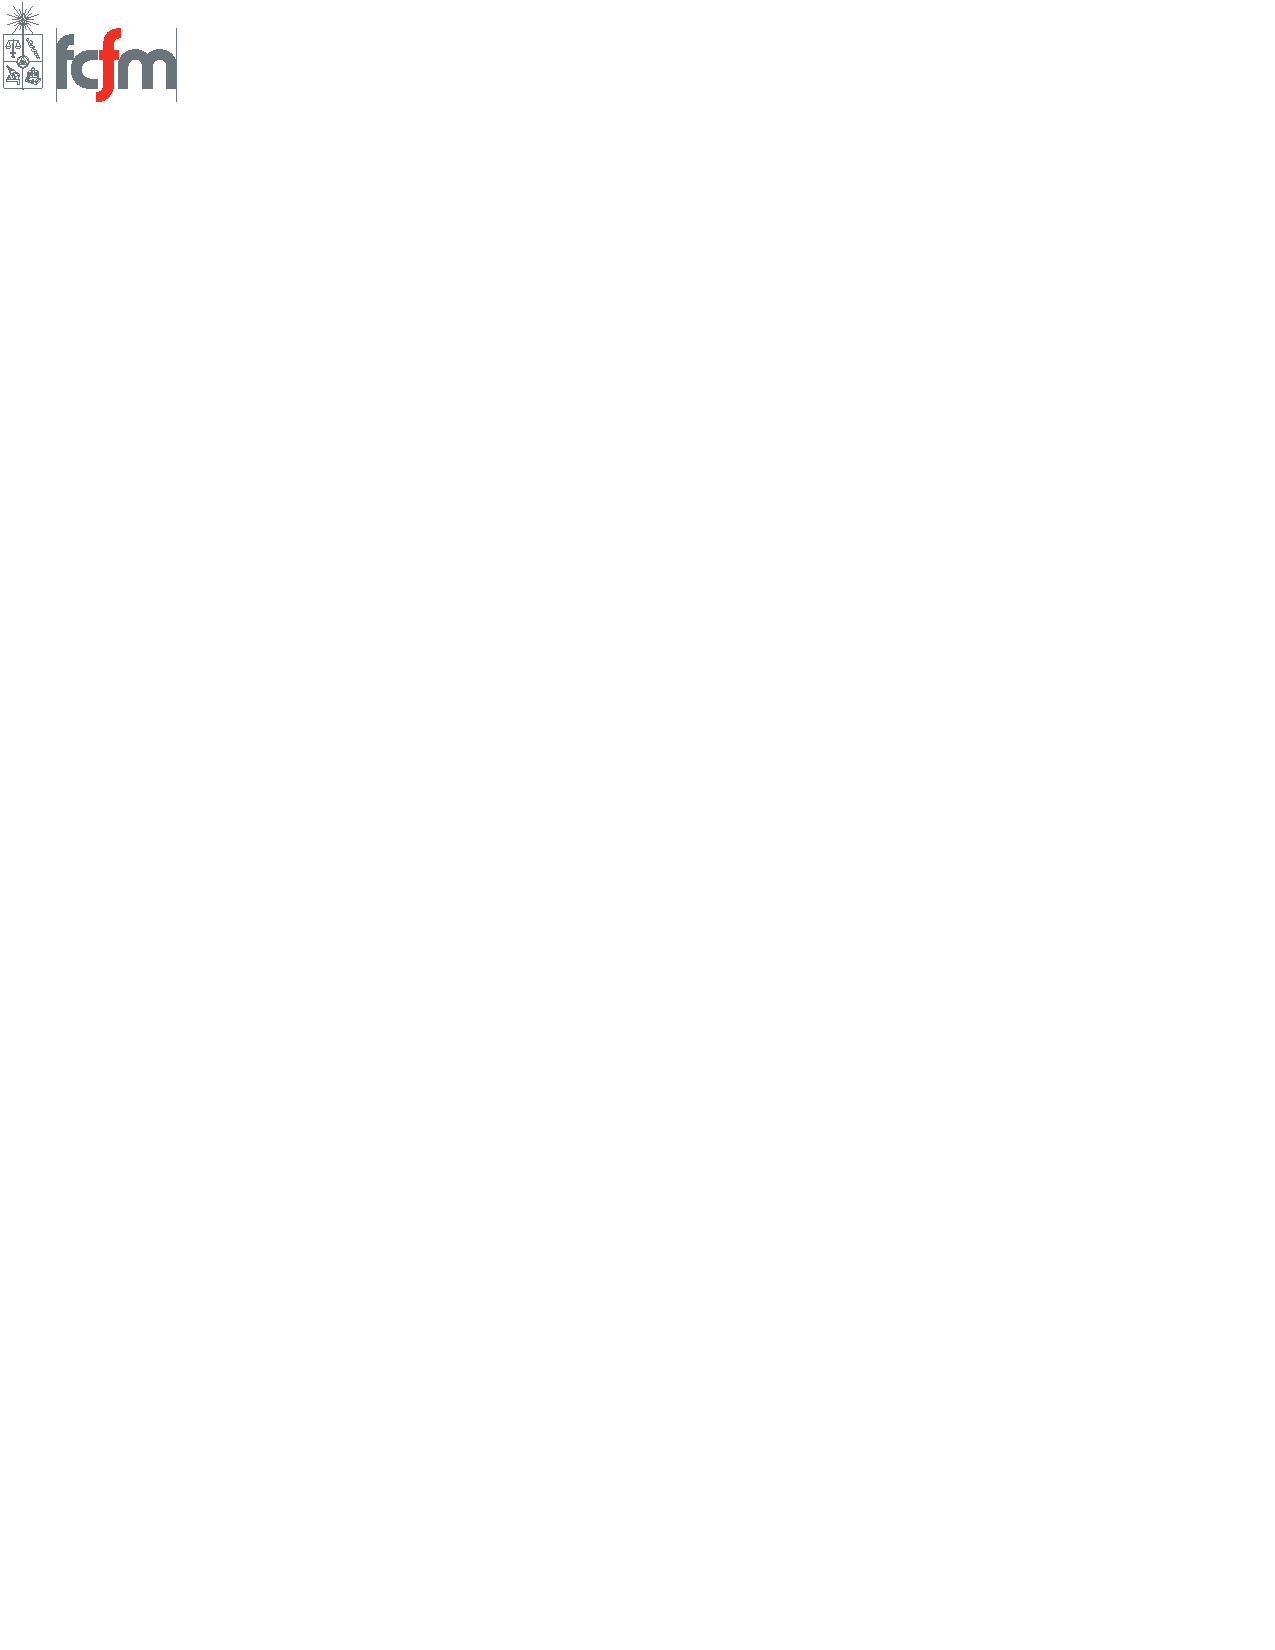
\includegraphics[scale=1.2]{fcfm2.pdf}}
\end{picture}

\begin{center}
	\LARGE \bf{Pauta Auxiliar \#3}\\
\end{center}

\vspace{-1cm}
\begin{enumerate}\setlength{\itemsep}{0.4cm}	
\item[]

\item Demostrar que si $A\subseteq \mathbb{R}^n $ es un cerrado o un abierto, entonces $\inte((\fr(A))=\phi$

\dem

\begin{itemize}
    \item A abierto:
    
    Razonando por contradicción: Tomemos $\inte(\fr(A))\neq\phi$
    
    Entonces $\exists x\in\inte(\fr(A))\Rightarrow (\exists \epsilon>0) B(x,\epsilon)\subseteq \fr(A)$ (*)
    
    Pero recordando que $\fr(A)=\adh(A)\backslash\inte(A)=\adh(A)\cap\inte(A)^c=adh(A)\cap A^c$, pues A es abierto 
    
    Entonces tenemos que $ B(x,\epsilon)\subseteq\adh(A)\cap A^c$, esto último implica que: $$\text{como } x\in B(x,\epsilon)\Rightarrow x\in\adh(A) \wedge \text{ }x\in A^c \text{, y en específico } x\in\adh(A)\Leftrightarrow (\forall r>0) B(x,r)\cap A\neq \phi$$
    Como la definición de adherencia se tiene para todo $r$, se tendrá para $\epsilon$, i.e: 
    $$B(x,\epsilon)\cap A\neq\phi \text{ (**)}$$ 
    
    Por otro lado, de (*): 
    \begin{align*}
        B(x,\epsilon)\subseteq&\adh(A)\cap A^c \text{  }\big{\slash}\cap A\\
        B(x,\epsilon)\cap A\subseteq&\adh(A)\cap A^c\cap A=\phi\\
        \Rightarrow& B(x,\epsilon)\cap A=\phi
    \end{align*}
    Llegando a una contradicción con (**)
    
    $\therefore$ para A abierto $\inte(\fr(A))=\phi$
    
    \item A cerrado:
    
    Notemos que $\fr(A)=\adh(A)\backslash\inte(A)=\adh(A)\cap\inte(A)^c=\adh(A)\cap\adh(A^c)$ por propiedad vista en auxiliar\#2, y usando la definición de adherencia se obtiene la siguiente definición de frontera:
    \[\fr(A)=\{x\in \mathbb{R}^n: (\forall r>0)\text{ } B(x,r)\cap A\neq\phi \wedge \text{ } B(x,r)\cap A^c\neq\phi\}\]
    
    A partir de estas definiciones es fácil apreciar que $\fr(A)=\fr(A^c)$.  De esta manera se tiene que $\inte(\fr(A))=\inte(\fr(A^c))$.
    
    Pero $A^c$ es abierto y, por la parte anterior se tiene que $\inte(\fr(A^c))=\phi$.
    
    $\therefore$ para A cerrado $\inte(\fr(A))=\phi$
    
    
\end{itemize}
\item Sea $(a_k)$ y $(b_k)$ dos sucesiones en $\mathbb{R}^n$, tales que $a_k\rightarrow a$ y $a_k+b_k\rightarrow c$. Demuestre  que $(b_k)$ es convergente.

\dem

Tenemos que $a_k\rightarrow a$ y $a_k+b_k\rightarrow c$, entonces notemos que:
\[b_k=b_k+a_k-a_k\Rightarrow \lim_{k\rightarrow\infty} b_k=\lim_{k\rightarrow\infty}(b_k+a_k-a_k)\]

Por álgebra de límites tenemos que:
\[\lim_{k\rightarrow\infty}b_k=\lim_{k\rightarrow\infty}(b_k+a_k)-\lim_{k\rightarrow\infty}(a_k)=c-a\]

\item Sea $y\in\mathbb{R}^n$ fijo y $r\in\mathbb{R}$. Muestre que el conjunto $A=\{x\in\mathbb{R}^n:\norm{x-y}\geq r\}$ es un conjunto cerrado mediante sucesiones.

\dem

Recordemos que $A \subseteq\mathbb{R}^n$ es cerrado ssi $\forall x_n\in A$ tal que $x_n\rightarrow x \Rightarrow x\in A$. 

Sea $x_n\in A$ tal que $x_n\rightarrow x$ \textit{PDQ.:} $x\in A$

$x_n\in A\Leftrightarrow \norm{x_n-y}\geq r$, pero $\norm{x_n-y}=\norm{x_n-y+x-x}=\norm{(x_n-x)+(x-y)}\leq \norm{x_n-x}+\norm{x-y}$. Entonces $r\leq \norm{x_n-x}+\norm{x-y} $

Tomando el límite:
\[r\leq\lim_{n\rightarrow\infty}(\norm{x_n-x}+\norm{x-y})=\norm{x-y}=\lim_{n\rightarrow\infty}\norm{x_n-x}+\norm{x-y}=\norm{x-y} \]
Entonces se tiene que $r\leq\norm{x-y}\Leftrightarrow x\in A$

$\therefore$ A es cerrado

pd: notar que el complemento del conjunto es una bola abierta, por lo que rápidamente se podía apreciar que el conjunto es cerrado.

\item Sea $E$ un e.v.n de dimensión finita (o $\R^d$ en su defecto) y $F\subseteq E$ un subespacio vectorial generado por el conjunto linealmente independiente $\{x_1,\ldots,x_m\}\subseteq E$, esto es, para cada $y\in F$ existen escalares $\lambda_1,\ldots,\lambda_m$ tal que
$y=\sum_{i=1}^m\lambda_i x_i $. Demuestre que $F$ es cerrado.

\dem 

Usaremos la caracterización por sucesiones: Sea $(y_n)_n\subseteq F$ una sucesión cualquiera tal que $y_n\to y\in E$, debemos probar que $y\in F$. Tenemos que para cada $n\in\N$, $y_n\in F$, por lo que podemos escribir
\[y_n=\sum_{i=1}^m\lambda_{i}^nx_i,\]
y notemos que si queremos probar que $y=\sum_{i=1}^m\lambda_i x_i $, necesariamente se debe cumplir que $\lambda_i^n\conv{n}{\infty}\lambda_i$ para cada $i=1,\ldots,m$. Con esta idea en mente, consideremos la sucesión definida por $\vec{\lambda}_n=(\lambda_1^n,\ldots,\lambda_m^n)\in\R^m$ y veamos que es acotada, pues en ese caso debe tener una subsucesión convergente \[\vec{\lambda}_{n_j}\conv{j}{\infty}\vec{\lambda}=(\lambda_1,\ldots,\lambda_m),\]
con lo cual 
\[y_{n_j}=\sum_{i=1}^m\lambda_{i}^{n_j}x_i\conv{j}{\infty} \sum_{i=1}^m\lambda_i x_i\]
y como $(y_{n_j})_j$ es subsucesión de $(y_n)_n$ que es convergente a $y$, necesariamente $y=\sum_{i=1}^m\lambda_i x_i\in F$, concluyendo que $F$ es cerrado.

Supongamos por contradicción que $(\vec{\lambda}_n)_n$ no es acotada, es decir que dada cualquier cota se puede encontrar algún elemento de la sucesión cuya norma supere dicha cota. En particular, para todo $j\in\N$, existe $\vec{\lambda}_{n_j}$ tal que $\norm{\vec{\lambda}_{n_j}}>j$, con lo cual formamos una sucesión real dada por $r_j=\norm{\vec{\lambda}_{n_j}}$ que cumple $r_j\conv{j}{\infty}\infty$. Ahora, como $(y_n)_n$ es una sucesión convergente, en particular es acotada y
\begin{equation}
    \frac{y_{n_j}}{r_j}=\underbrace{\frac{1}{r_j}}_{\text{nula}}\underbrace{y_{n_j}}_{\text{acotada}}\conv{j}{\infty} 0. 
\end{equation}
Por otro lado
\[\frac{y_{n_j}}{r_j}=\frac{1}{r_j}\sum_{i=1}^m \lambda_i^{n_j}x_i=\sum_{i=1}^m \frac{\lambda_i^{n_j}}{r_j}x_i \]
y podemos notar que los coeficientes de la expresión anterior son las componentes de la sucesión $\Big(\frac{\vec{\lambda}_{n_j}}{r_j}\Big)_j$ que vive en la frontera de la bola unitaria:
\[\bigg\lVert\frac{\vec{\lambda}_{n_j}}{r_j}\bigg\rVert
=\frac{\norm{\vec{\lambda}_{n_j}}}{r_j}=1.\]

Luego, $\Big(\frac{\vec{\lambda}_{n_j}}{r_j}\Big)_j$ es acotada, por lo que tiene una subsucesión convergente (sin pérdida de generalidad y para evitar sobrecargar notación diremos que ella misma converge) a algún $\vec{\mu}=(\mu_1,\ldots,\mu_m)\in\fr(B(0,1))\subseteq\R^m$, donde ocupamos el hecho que la frontera es un conjunto cerrado. Con esto,
\[\frac{y_{n_j}}{r_j}=\sum_{i=1}^m \frac{\lambda_i^{n_j}}{r_j}x_i\conv{j}{\infty}\sum_{i=1}^m\mu_ix_i,\]
pero juntando esto con lo que vimos en (1), tenemos que $\sum_{i=0}^m\mu_ix_i=0$ con $\mu\neq0$ (porque $0\notin \fr(B(0,1))$, lo cual contradice la independencia lineal del conjunto $\{x_1,\ldots,x_m\}$. Luego, $(\vec{\lambda}_n)_n$ debe ser acotada.

\end{enumerate}	
\end{document}